%dev_3.tex
%Par Guillaume Lahaie
%LAHG04077707
%
%%%%%%%%%%%%%%%%%%%%%%%%%%%%%%%%%%%%%%%%%
% Simple Sectioned Essay Template
% LaTeX Template
%
% This template has been downloaded from:
% http://www.latextemplates.com
%
% Note:
% The \lipsum[#] commands throughout this template generate dummy text
% to fill the template out. These commands should all be removed when 
% writing essay content.
%
%%%%%%%%%%%%%%%%%%%%%%%%%%%%%%%%%%%%%%%%%

%----------------------------------------------------------------------------------------
%	PACKAGES AND OTHER DOCUMENT CONFIGURATIONS
%----------------------------------------------------------------------------------------

\documentclass[10.9pt]{article} % Default font size is 12pt, it can be changed here
\renewcommand{\familydefault}{\rmdefault}
\renewcommand{\thesubsection}{\alph{subsection}}

%Pour l'encodage avec accents
\usepackage[utf8]{inputenc}
\usepackage{longtable}
\usepackage{algorithm2e}

%\usepackage{helvet}
%\renewcommand{\familydefault}{\sfdefault}

%Pour INF4100 - devoir 3
\usepackage{tikz}
\usepackage{algorithm2e}

\usepackage{afterpage}
\usepackage{appendix}
\usepackage{graphics} % Required for including pictures
\usepackage{listings}
\usepackage{mathtools}

\usepackage[left=2.2cm,top=2.2cm,right=2.2cm,bottom=2.2cm,nohead]{geometry} % Required to change the page size to A4
\geometry{letterpaper} % Set the page size to be A4 as opposed to the default US Letter

\usepackage{float} % Allows putting an [H] in \begin{figure} to specify the exact location of the figure
\linespread{1.2} % Line spacing

%\setlength\parindent{0pt} % Uncomment to remove all indentation from paragraphs

\graphicspath{{./Pictures/}} % Specifies the directory where pictures are stored
\usepackage[french,english]{babel}

%Comportement d'un paragraphe
\setlength{\parskip}{\baselineskip}%
\setlength{\parindent}{0pt}%

%Widows/orphans
\widowpenalty10000
\clubpenalty10000

\usepackage[hidelinks]{hyperref}

%Meta-info
\title{INF4100 - devoir 3}
\author{Guillaume Lahaie}
\date{Remise: 1er avril 2014}

\hypersetup{
  pdftitle={INF4100 - devoir 3},
  pdfauthor={Guillaume Lahaie}
}

\newcommand\blankpage{%
  \null
  \thispagestyle{empty}%
  \addtocounter{page}{-1}%
  \newpage}

\begin{document}
\selectlanguage{french}
\fussy

%----------------------------------------------------------------------------------------
%	TITLE PAGE
%----------------------------------------------------------------------------------------

\begin{titlepage}

\newcommand{\HRule}{\rule{\linewidth}{0.5mm}} % Defines a new command for the horizontal lines, change thickness here

\center % Center everything on the page

\textsc{\LARGE Université du Québec à Montréal}\\[1.5cm] % Name of your university/college
\textsc{\Large INF4100}\\[0.5cm] % Major heading such as course name

\HRule \\[1.5cm]
{ \huge \bfseries Devoir 3}\\[0.4cm] % Title of your document
\HRule \\[1.5cm]

\begin{minipage}{0.4\textwidth}
\begin{flushleft} \large
\emph{Par:}\\
Guillaume Lahaie \\ LAHG04077707 % Your name
\end{flushleft}
\end{minipage}
~
\begin{minipage}{0.4\textwidth}
\begin{flushright} \large
\emph{Remis à:} \\
Louise Laforest % Supervisor's Name
\end{flushright}
\end{minipage}\\[4cm]

{\large \emph{Date de remise:} \\ Le 1$^{er}$ avril 2014}\\[3cm] % Date, change the \today to a set date if you want to be precise

%\includegraphics{Logo}\\[1cm] % Include a department/university logo - this will require the graphicx package

\vfill % Fill the rest of the page with whitespace

\end{titlepage}
\blankpage

%----------------------------------------------------------------------------------------
%	TABLE OF CONTENTS
%----------------------------------------------------------------------------------------

\tableofcontents % Include a table of contents

\newpage % Begins the essay on a new page instead of on the same page as the table of contents 

%----------------------------------------------------------------------------------------
% SECTIONS DU DOCUMENT
%----------------------------------------------------------------------------------------


\section{Numéro 1.}

\subsection{Concevez une fonction qui prend en entrée deux matrices et qui
            retourne le resultat de la multiplicationd des matrices}
            
Voir la fonction \texttt{multiplierMatrice} du fichier \texttt{matrices.py}.

\subsection{Implantez l'algorithme naïf}

Voir la fonction \texttt{trouverParenthesageOptimalNaif} du fichier \texttt{matrices.py}.

\subsection{Implantez l'algorithme naïf avec stockage des calculs déjà effectués}

Voir la fonction \texttt{trouverParenthesageOptimalAvecStockage} du fichier \texttt{matrices.py}.

\subsection{Implantez l'algorithme de programmation dynamique}

Voir la fonction \texttt{trouverParenthesageOptimalDynamique} du fichier \texttt{matrices.py}.

\subsection{Comparez les temps d'exécution des trois algorithmes}

J'ai d'abord fait un premier test pour des chaines de matrices contenant de
5 à 20 matrices à multiplier.

Le premier
graphique présente les resultats pour les trois algorithmes, pour une chaine
de matrices variant de 5 à 20 matrices. Le second graphique présente les
résultats pour l'algorithme de programmation dynamique et l'algorithme
diviser pour régner avec stockage.

Le premier graphique démontre que pour l'algorithme naïf, le temps d'exécution s'accroit
de façon exponentiel, et donc après 20 matrices, le temps d'exécution
devient trop long pour représenter sur le graphique.

On peut voir ensuite que le temps d'exécution pour l'algorithme diviser
pour régner avec stockage et l'algorithme en programmation dynamique
croit à un rythme similaire.

L'algorithme naif avec stockage est un peu moins efficace, car il est toujours
récursif. De plus, il faut toujours vérifier si le résultat partiel est
déjà disponible ou non.

J'ai ensuite créer un script pour tester la performance des algorithmes (\texttt{test\_performance.py}).
Ce script prend en entrée un nombre de matrices dans une chaine, et calcule le parenthésage optimal
avec les trois algorithmes. Si les temps d'exécution dépasse 5 secondes, le calcule est annulé.

On peut remarquer ici que plus le même résultat que pour le premier test, le temps d'exécution de
l'algorithme naïf croit exponentiellement, alors que les deux autres algorithmes croissent au 
même rythme.

\begin{center}
 \includegraphics[angle=270,scale=0.5]{resultat.eps}
 \includegraphics[angle=270,scale=0.5]{resultat2.eps}
\end{center}

\newpage
\subsection{Algorithme qui affiche l'expression de parenthésage}\label{parenthesage}

Cet algorihtme vient du livre \emph{Introduction to Algorithms, 3rd edition}, de
Cormen, Leiserson, Rivest, Stein:

\begin{algorithm}
 \SetKwInput{Donnees}{donnees}
 \SetKwInput{Antecedents}{antécédents}
 \SetKwInput{Consequents}{conséquents}
 \SetKwInput{Fonction}{fonction}
 \Fonction{imprimerParenthesage($frontiere, i, j$)}
 \Donnees{ \emph{frontiere}: matrice n*n indicé de 1 à $n$ \\ 
	   \emph{i}: un indice entre 1 et $n$ \\
	   \emph{j}: un indice entre 1 et $n$}
 \Consequents{Le parenthésage optimal est affiché à l'écran}
 \Deb{
    \Si{$ i == j$}{
	imprimer("A"+$i$)
	}
      \Sinon{
	imprimer("(")\\
        imprimerParenthesage($frontiere$, $i$, $frontiere[i][j]$)\\
        imprimerParenthesage($frontiere$, $frontiere[i][j]+1$, $j$)\\
        imprimer(")")\\
        }
    }       
\end{algorithm}

L'algorithme est implémenté dans la fonction \texttt{afficherParenthesageOptimal} du
fichier \texttt{matrices.py}.

\subsection{Algorithme qui multiplie la suite de matrices selon la matrice frontiere}

\subsubsection{Algorithme}

Cet algorithme est basé sur l'algorithme de parenthésage en \ref{parenthesage}.

\begin{algorithm}
 \SetKwInput{Donnees}{donnees}
 \SetKwInput{Antecedents}{antécédents}
 \SetKwInput{Consequents}{conséquents}
 \SetKwInput{Fonction}{fonction}
 \Fonction{multiplierChaineMatrices($matrices, frontiere, i, j$)}
 \Donnees{ \emph{matrices}: chaine de matrices à multiplier
	   \emph{frontiere}: matrice n*n indicé de 1 à $n$ \\ 
	   \emph{i}: un indice entre 1 et $n$ \\
	   \emph{j}: un indice entre 1 et $n$}
 \Sortie{Le résultat de la multiplication de la chaine de matrices}
 \Deb{
    \Si{$ i == j$}{
	retourner $matrices[i]$
	}
      \Sinon{
	$c$ $\longleftarrow$ multiplierChaineMatrices($matrices, frontiere, i, frontiere[i][j]$)\\
	$d$ $\longleftarrow$ multiplierChaineMatrices($matrices, frontiere, frontiere[i][j]+1, j$)\\
	\Retour{multiplierMatrice(c, d)}
        }
    }       
\end{algorithm}

Cet algorithme est implémenté par la fonction \texttt{multiplierChaineMatrice} du fichier \texttt{matrices.py}.

\subsubsection{Analyse de la complexité temporelle de l'algorithme}

On connait déjà le nombre de multiplications totales à effectuer pour mutiplier la chaine de matrices. En effet,
il s'agit du résultat de l'algorithme de parenthésage utilisé.

On peut donc dire de façon précise le nombre de multiplications scalaires totales qui seront effectuées. 
Toutefois, cela ne donne pas la complexité temporelle de l'algorithme.

Une autre approche serait de considérer que la multiplication de matrices à comme complexité temporelle $O(n^3)$, 
où $n$ représente la grandeur maximale d'une des deux matrices à multiplier (par exemple, le nombre de ligne de
la matrice A, le nombre de colonnes de B, ou le nombre de colonnes de A).

Si nous avons $m$ matrices dans la chaine, nous aurons donc $m-1$ multiplications de matrices à effectuer.
Donc, si chaque multiplication a comme complexité temporelle $O(n^3)$, alors la complexité temporelle
de la multiplication de la chaine sera:

$T(n) = O((m-1)n^3) = O(mn^3)$, où $m$ est le nombre de matrices à multiplier, et $n$ la dimension maximale
d'une matrice dans la chaine.

\end{document}
